\documentclass[root.tex]{subfiles}

\begin{document}

{\pagestyle{empty}}
\section{Software-Setup}
\label{chap:Software-Setup}
In this section a short overview of the utilized software and its interdependencies shall be given. 

\subsection{\gls{VTM}}

To evaluate the dynamic performance of the \gls{HCT}-combination Volvo's \gls{VTM} came to use. It is a library developed in and for Simulink and permits the simulation of truck dynamics based on a multi-body model for the kinematic relation and a parametrized tire model around the magic formula. Many different \gls{HCT}-combinations, road-situations and maneuver definitions come pre-defined with the tool-kit enabling a fairly quick implementation of full vehicle simulations. 

\subsection{RTI-blockset}

dSpace's rapid-prototyping platform's connection with Simulink is centered around a library which provides access to all physical communication ports on the \gls{MABII}, real-time execution on the target hardware and straight forward code-generation and -download. It was used to implement the \gls{CAN}-communication with the \gls{ETS}, the \gls{EBS} and will be used to incorporate more signals from the truck's chassis-\gls{CAN} in the future. Another use of the block-set was to ensure \gls{UDP}-communication within the \gls{HIL}-testing, as the Ethernet-port on the \gls{MABII} was used to supply data from the hardware system to the simulated sub-systems.

\subsection{ControlDesk}

As the simulation is executed on the \gls{MABII} it is possible to access representations of all blocks and their values and properties that are part of the abstract Simulink model which was generated to the \gls{MABII}. It thus is possible to have a user-readable system-state monitor. A number of \gls{GUI} creation tools permit fast development. During execution ControlDesk runs on a standard PC, which accesses the \gls{MABII}'s RAM via ethernet connection. 

%\begin{figure}
%\centering
%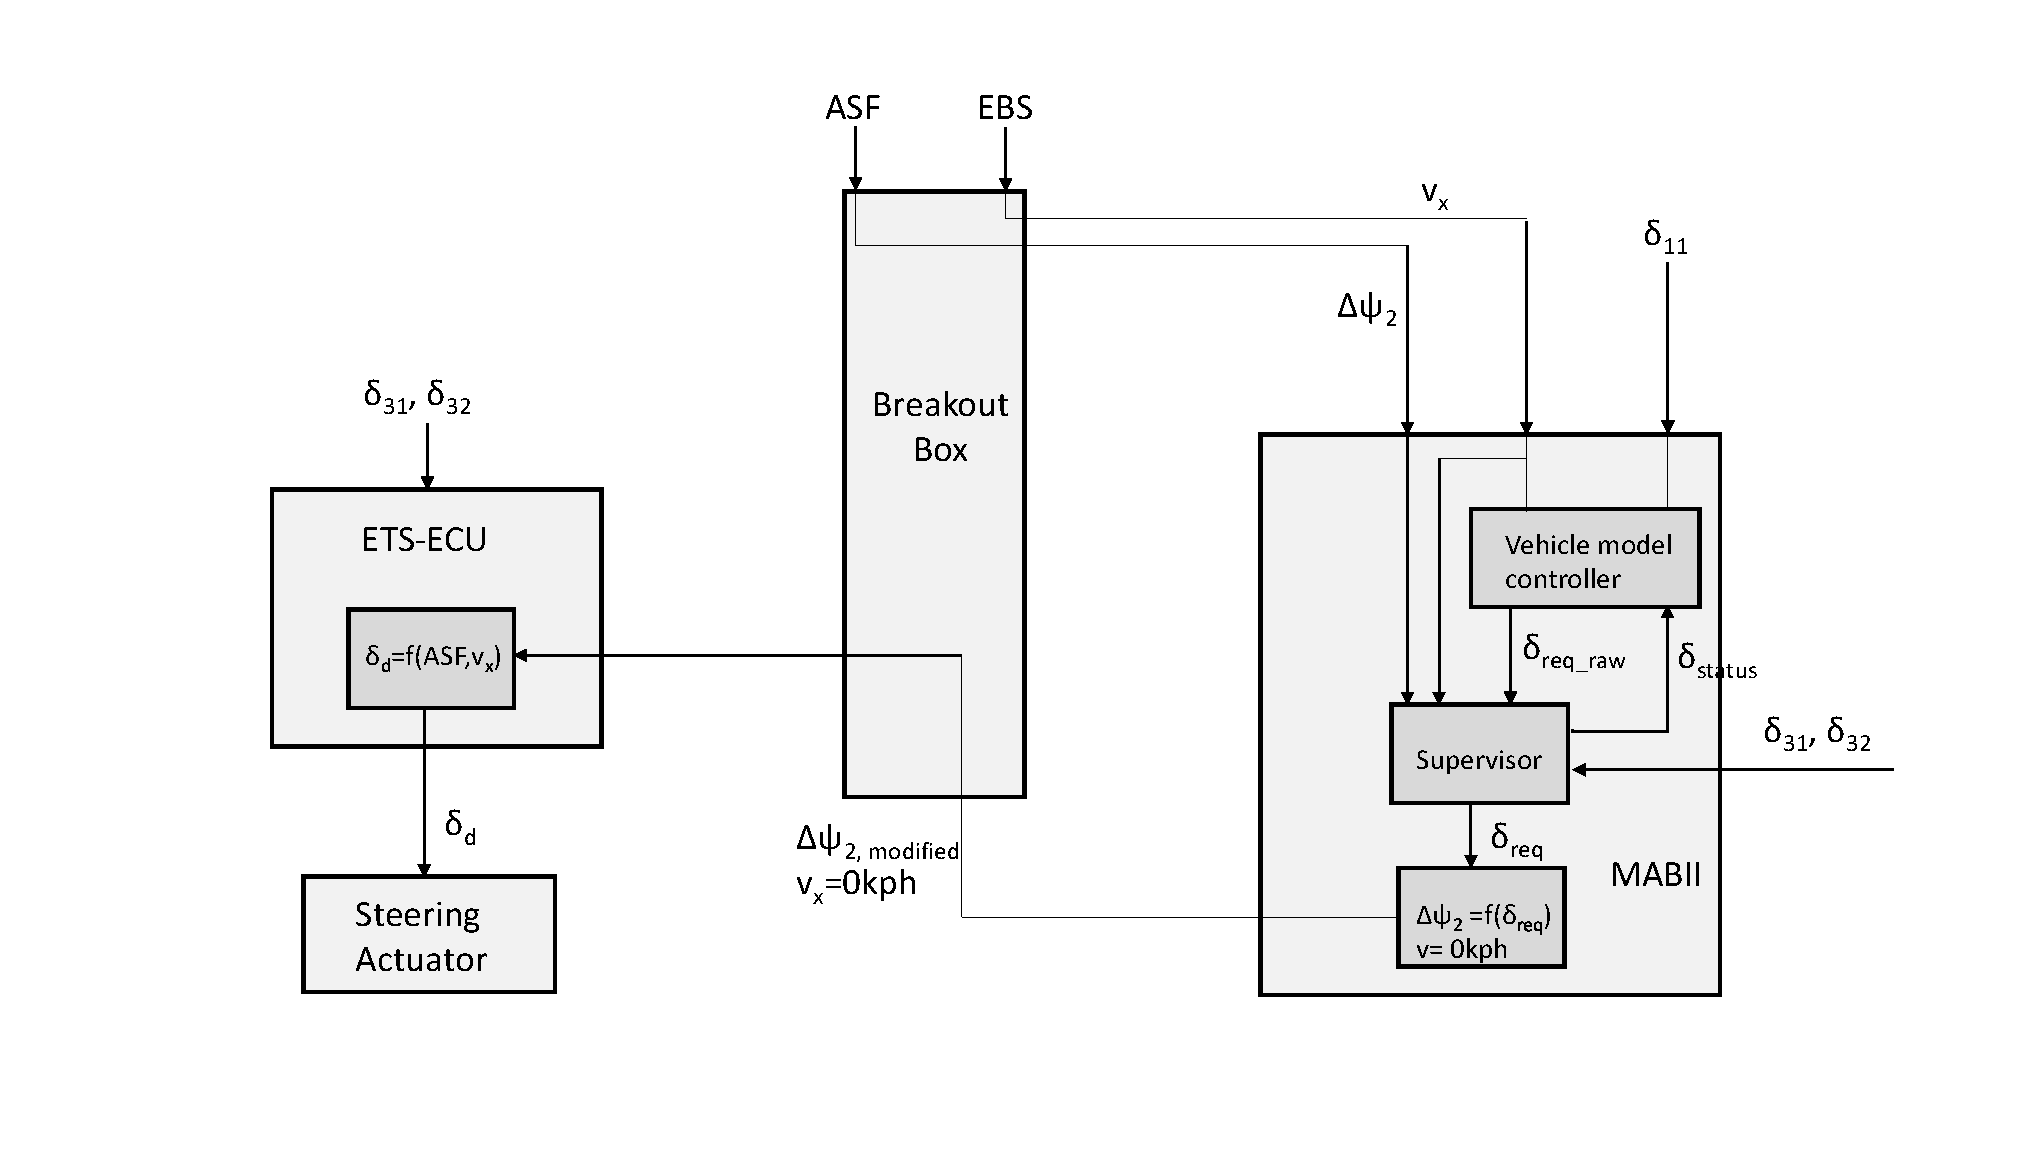
\includegraphics[width=1\linewidth]{system_mod}
%\caption{Signal path overview for modified \gls{ETS}}
%\label{fig:system_mod}
%\end{figure}
\end{document}